\chapter{Declension Table}\label{chap:decl}

This is one of the most useful tools for new learners. Traditional students have to remember many of these tables. While remembering some key paradigms is still important in learning process, this tool can enhance your ability to search and experiment in just a few clicks. The Declension window can be opened by menu Grammar > {\faSix \symbol{"F00A}} Declension\,table. The results of Declension table can be grouped into three: nouns and adjectives, pronouns, and numbers.

\section{Pronouns}

For new users, seeing \emph{Pronouns} first is easier because the pronoun list is finite and it is often used. You will see something like Figure \ref{fig:declension-pron}. The result of declension tables will show one gender at a time. If there are multiple genders to decline, you can choose whether \emph{m} (masculine), \emph{f} (feminine), or \emph{nt} (neuter). Short meaning of each pronoun can also be added when this option is selected.

\begin{figure}[!hbt]
\centering
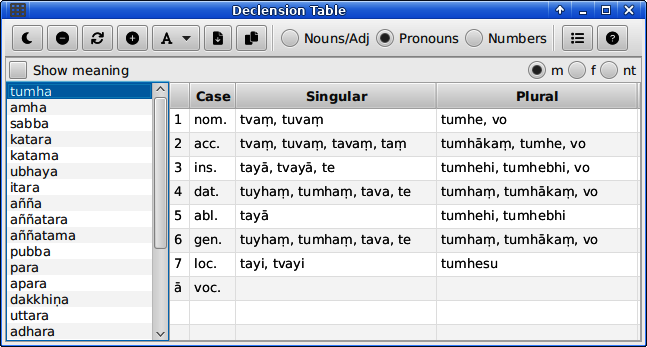
\includegraphics[width=0.9\linewidth]{images/declension-pron.png}\\
\caption{Declension table of a pronoun}
\label{fig:declension-pron}
\end{figure}

To remind new students, the expansion of abbreviations used in the table, as shown in Table \ref{tab:cases-expanded}, may do some help. Note that some of pronouns have no vocative form, so the row of this is blank.

\begin{table}[!hbt]
\centering
\caption{Expansion of case abbreviations}
\label{tab:cases-expanded}
\bigskip
\begin{tabular}{lll} \toprule
1 & paṭhamā & nominative case \\
2 & dutiyā & accusative case \\
3 & tatiyā & instrumental case \\
4 & catutthī & dative case \\
5 & pañcamī & ablative case \\
6 & chaṭṭhī & genitive case \\
7 & sattamī & locative case \\
ā & ālapana & vocative case \\
\bottomrule
\end{tabular}
\end{table}

An amazing feature of this tool is that you can check the declined terms against a term list in the text collections. When {\faSix \symbol{"F03A}} button is hit, you will see the right pane opened (see Figure \ref{fig:declension-pron-list}). If you have ever generated a table of term list (see Chapter \ref{chap:lister}), there will be a term-frequency list able to check against the data displayed. Then, you can know which forms are actually used in the texts (of a specified collection). Remember that one declined form of a Pāli word can come from different bases, for example \pali{taṃ} and \pali{te} may come from \pali{tumha} or \pali{ta}.

\begin{figure}[!hbt]
\centering
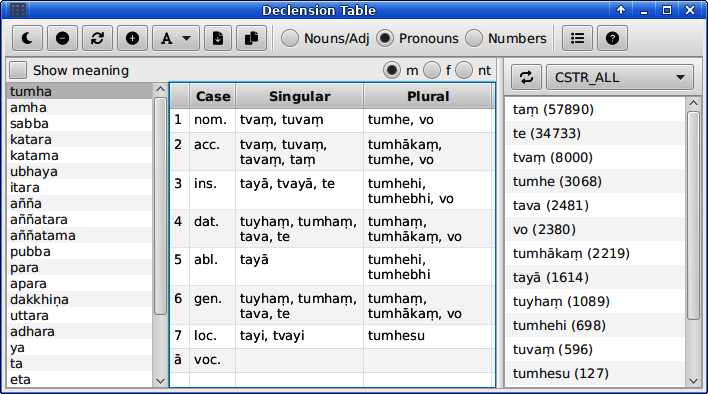
\includegraphics[width=0.9\linewidth]{images/declension-pron-list.png}\\
\caption{Declension of \pali{tumha} against a term-freq list}
\label{fig:declension-pron-list}
\end{figure}

\section{Nouns/Adjectives}

Nouns and adjectives in Pāli undergo the same inflectional rules, and sometimes a word takes dual position. So, I group them together. Since terms in this group are numerous, you can select what you want to see by entering some query. Only simple search is available here. The source of terms is the \emph{Concise Pāli-English Dictionary} (CPED). An example of noun's declension is shown in Figure \ref{fig:declension-noun}. 

\begin{figure}[!hbt]
\centering
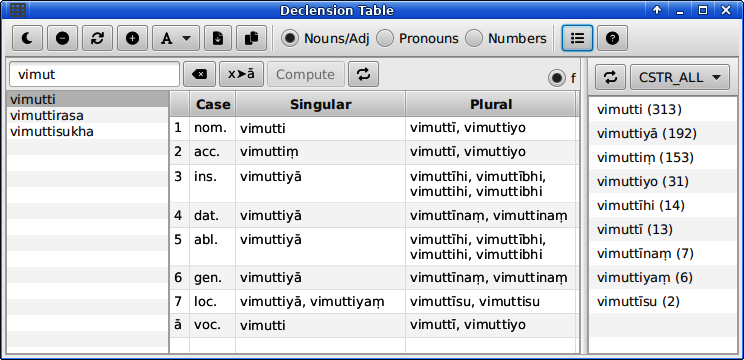
\includegraphics[width=0.9\linewidth]{images/declension-noun-list.png}\\
\caption{Declension of \pali{vimutti} against a term-freq list}
\label{fig:declension-noun}
\end{figure}

Results of an adjective's declension look exactly the same, but adjectives can be declined into all three genders.

What about the \emph{Compute} button then? It has two uses. First, when a term has both regular and irregular declensions. And second, just when you want to play around with experiments.

I will give an example of the first case. For the second, the users can do by themselves. There are many words that use irregular paradigms, and I put a lot of effort to incorporate them here seamlessly.\footnote{If you find any irregular word that is declined wrongly according to the traditional textbooks, please report to the author right away.}

A term I give here is \pali{sara}. When it means `pond' it is declined irregularly as \pali{mano-gaṇa} (m.\ only). This is what is shown when you enter \pali{`sara'} at the search box. But when it means `sound' or `arrow' it is declined like a normal noun (m.\ and nt.). To reach the latter case you have to hit \emph{Compute} after you enter \pali{`sara'}. See the comparison in Figure \ref{fig:declension-sara-compare}.

\begin{figure}[!hbt]
\centering
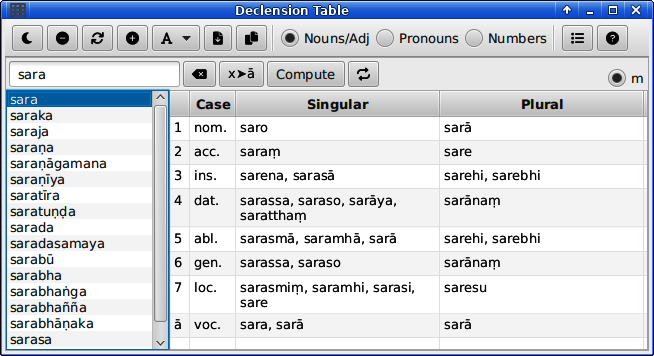
\includegraphics[width=0.9\linewidth]{images/declension-sara-mano.png}\\
(a) Declined as \pali{mano-gaṇa}\\[3mm]
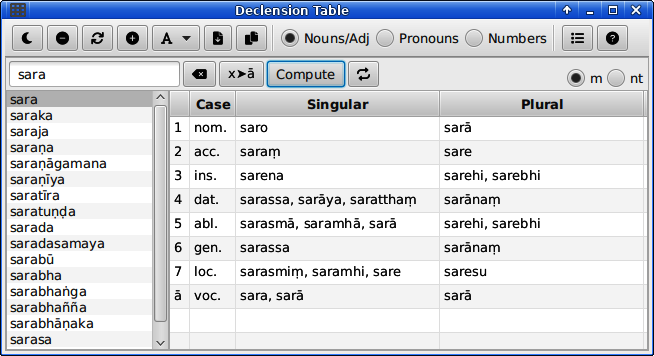
\includegraphics[width=0.9\linewidth]{images/declension-sara-compute.png}\\
(b) Computed declension (normal noun)\\
\caption{Declension of \pali{sara} in two cases}
\label{fig:declension-sara-compare}
\end{figure}

For those who want to experiment with generic paradigms, you simply input a word with a proper ending and hit \emph{Compute}. The proper endings are \pali{a, i, ī, u, ū} for masculine words, \pali{ā, i, ī, u, ū} for feminine words, and \pali{a, i, u} for neuter words. There are also two exceptions which use their special paradigms: \mbox{\pali{-ant}} (like \pali{himavant} or \pali{himavantu}) and \pali{-ar} (like \pali{kattar} or \pali{kattu}).

\boxnote{When experimenting with declensional paradigms, there are two special cases:\\
\hspace{5mm}(1) Stems ending with \pali{-ant} decline irregularly like \pali{himavant} or \pali{himavantu}\\
\hspace{5mm}(2) Stems ending with \pali{-ar} decline irregularly like \pali{kattar} or \pali{kattu}
}

\section{Numbers}

Numeral declension is one of the most difficult parts of the program to implement.\footnote{The code of this part is not long but complicated.} All output in this part comes from calculation. That means you can enter any number up to 6 digits, and it will be converted to its Pāli numeral\footnote{The result list is not exhaustive, because one complex number can be rendered in many ways. The results here show only some compound units that can be calculated by computation. Try 150, 250, 350, and so on; you will see why the conversion is so difficult.} with declension tables, both cardinal and ordinal. To help the beginners, however, there are pre-built lists that can be easily selected. Figure \ref{fig:declension-num} shows the result of \texttt{100250}.

I will skip other details because everything is self-explained and it is better to learn by playing.

\newpage
\begin{figure}[!hbt]
\centering
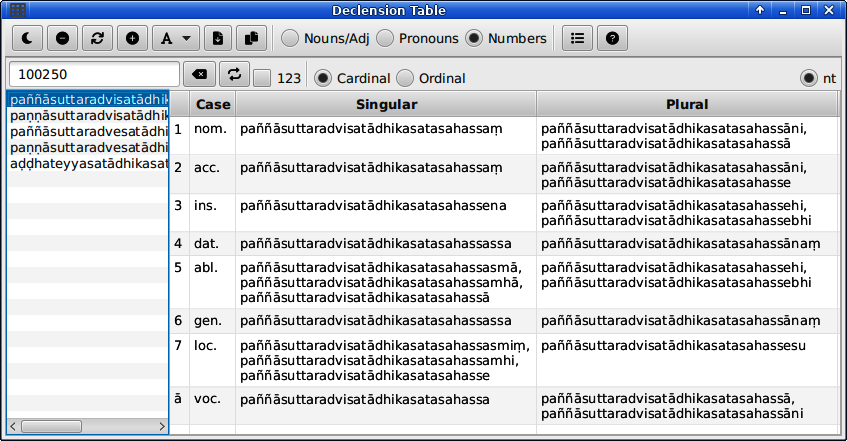
\includegraphics[width=0.9\linewidth]{images/declension-num.png}\\
\caption{Declension of \texttt{100250}}
\label{fig:declension-num}
\end{figure}

